\underline{Exercise 7.1}
\begin{enumerate}
% Question 3
\item[3.]
\begin{enumerate}
\item[(a)] $f^{\prime}(x)=18$, so $f^{\prime}(1)=18$ and $f^{\prime}(2)=18$.
\item[(b)] $f^{\prime}(x)=3 c x^{2}$, so $f^{\prime}(1)=3 c$ and $f^{\prime}(2)=12 c$.
\item[(c)] $f^{\prime}(x)=10 x^{-3}$, so $f^{\prime}(1)=10$ and $f^{\prime}(2)=\frac{10}{8}=\frac{5}{4}$.
\item[(d)] $f^{\prime}(x)=x^{1 / 3}=\sqrt[3]{x}$, so $f^{\prime}(1)=1$ and $f^{\prime}(2)=\sqrt[3]{2}$.
\item[(e)] $f^{\prime}(w)=2 w^{-2 / 3}$, so $f^{\prime}(1)=2$ and $f^{\prime}(2)=2 \cdot 2^{-2 / 3}=2^{1 / 3}$.
\item[(f)] $f^{\prime}(w)=\frac{1}{2} w^{-7 / 6}$, so $f^{\prime}(1)=\frac{1}{2}$ and $f^{\prime}(2)=\frac{1}{2} \cdot 2^{-7 / 6}=2^{-13 / 6}$.
\end{enumerate}
\end{enumerate}

\underline{Exercise 7.2}
\begin{enumerate}
% Question 3
\item[3.]
\begin{enumerate}
\item[(d)] Let $f(x)=a x-b$ and $g(x)=c x^{2}$, so $f^{\prime}(x)=a$ and $g^{\prime}(x)=2 c x$.
\[
\begin{aligned}
\frac{d}{d x}\left[f(x) g(x)\right] &=f^{\prime}(x) g(x)+f(x) g^{\prime}(x) \\
&=a c x^{2}+(a x-b) 2 c x \\
&=a c x^{2}+2 a c x^{2}-2 b c x \\
&=3 a c x^{2}-2 b c x
\end{aligned}
\]
\item[(e)] Let $f(x)=(2-3 x)(1+x)$ and $g(x)=x+2$, so $g^{\prime}(x)=1$. Using the product rule on $f(x)$ itself:
\[ f^{\prime}(x)=-3(1+x)+(2-3 x)(1)=-(6 x+1) \]
Then
\[
\begin{aligned}
\frac{d}{d x}\left[f(x) g(x)\right] &=f^{\prime}(x) g(x)+f(x) g^{\prime}(x) \\
&=-(6 x+1)(x+2)+(2-3 x)(1+x) \\
&=-6 x^{2}-13 x-2+2-x-3 x^{2} \\
&=-9 x^{2}-14 x=-x(9 x+14)
\end{aligned}
\]
\end{enumerate}

% Question 7
\item[7.]
\begin{enumerate}
\item[(a)] With $f(x)=x^{2}+3$, $f^{\prime}(x)=2 x$, and $g(x)=x$, $g^{\prime}(x)=1$:
\[
\begin{aligned}
\frac{d}{d x} \frac{f(x)}{g(x)} &=\frac{f^{\prime}(x) g(x)-f(x) g^{\prime}(x)}{g(x)^{2}} \\
&=\frac{(2 x) x-\left(x^{2}+3\right) \cdot 1}{x^{2}}=\frac{x^{2}-3}{x^{2}}
\end{aligned}
\]
\item[(b)] \[ \frac{d}{d x} \frac{x+9}{x}=\frac{1 \cdot x-1 \cdot(x+9)}{x^{2}}=\frac{-9}{x^{2}} \]
\item[(c)] \[ \frac{d}{d x} \frac{6 x}{x+5}=\frac{6(x+5)-1 \cdot 6 x}{(x+5)^{2}}=\frac{30}{(x+5)^{2}} \]
\item[(d)]
\[
\begin{aligned}
\frac{d}{d x} \frac{a x^{2}+b}{c x+d} &=\frac{2 a x(c x+d)-\left(a x^{2}+b\right) c}{(c x+d)^{2}} \\
&=\frac{2 a c x^{2}+2 a d x-a c x^{2}-b c}{(c x+d)^{2}} \\
&=\frac{a c x^{2}+2 a d x-b c}{(c x+d)^{2}}
\end{aligned}
\]
\end{enumerate}

% Question 8
\item[8.] $f(x)=a x+b$
\begin{enumerate}
\item[(a)] $f^{\prime}(x)=a$
\item[(b)] $\frac{d}{d x}\left(a x^{2}+b x\right)=2 a x+b$
\item[(c)] \[ \frac{d}{d x} \frac{1}{a x+b}=\frac{0 \cdot(a x+b)-a \cdot 1}{(a x+b)^{2}}=\frac{-a}{(a x+b)^{2}} \]
\item[(d)] \[ \frac{d}{d x} \frac{a x+b}{x}=\frac{a x-(a x+b) \cdot 1}{x^{2}}=\frac{-b}{x^{2}} \]
\end{enumerate}
\end{enumerate}

\underline{Exercise 7.3}
\begin{enumerate}
% Question 1
\item[1.]
\[ \frac{d y}{d u}=3 u^{2}+2 \qquad \frac{d u}{d x}=-2 x \]
\[ \frac{d y}{d x}=\frac{d y}{d u} \cdot \frac{d u}{d x}=\left(3 u^{2}+2\right)(-2 x)=-2 x\left[3\left(5-x^{2}\right)^{2}+2\right] \]

% Question 2
\item[2.]
\[
\begin{aligned}
\frac{d w}{d x} &=\frac{d w}{d y} \cdot \frac{d y}{d x} \\
&=2 a y(2 b x+c) \\
&=2 a\left(b x^{2}+c x\right)(2 b x+c)
\end{aligned}
\]

% Question 3
\item[3.]
\begin{enumerate}
\item[(a)] Let $z=3 x^{2}-13$, so $y=z^{3}$:
\[ \frac{d y}{d x}=\frac{d y}{d z} \cdot \frac{d z}{d x}=3 z^{2}(6 x)=18 x\left(3 x^{2}-13\right)^{2} \]
\item[(b)] Let $z=7 x^{3}-5$, so $y=z^{9}$:
\[ \frac{d y}{d x}=\frac{d y}{d z} \cdot \frac{d z}{d x}=9 z^{8}\left(21 x^{2}\right)=189 x^{2}\left(7 x^{3}-5\right)^{8} \]
\item[(c)] Let $z=a x+b$, so $y=z^{5}$:
\[ \frac{d y}{d x}=\frac{d y}{d z} \cdot \frac{d z}{d x}=5 z^{4}(a)=5 a(a x+b)^{4} \]
\end{enumerate}

% Question 4
\item[4.] Chain rule, with $z=16 x+3$ and $y=z^{-2}$:
\[ \frac{d y}{d x}=\frac{d y}{d z} \cdot \frac{d z}{d x}=-2 z^{-3}(16)=\frac{-32}{(16 x+3)^{3}} \]
Quotient rule, where the derivative of the denominator is $2(16 x+3) \cdot 16=32(16 x+3)$:
\[ \frac{d y}{d x}=\frac{0 \cdot(16 x+3)^{2}-1 \cdot 32(16 x+3)}{(16 x+3)^{4}}=\frac{-32}{(16 x+3)^{3}} \]
The answers are identical.

% Question 5
\item[5.] The inverse function is $x=\frac{y-21}{7}$.
\[ \frac{d y}{d x}=7 \qquad \frac{d x}{d y}=\frac{1}{7}=\frac{1}{d y / d x} \]
so the inverse-function rule holds. To graph the inverse with its own independent variable on the horizontal axis, write it as $y=(x-21)/7$. The two lines are mirror images of each other across the 45-degree line $y=x$:

\begin{center}
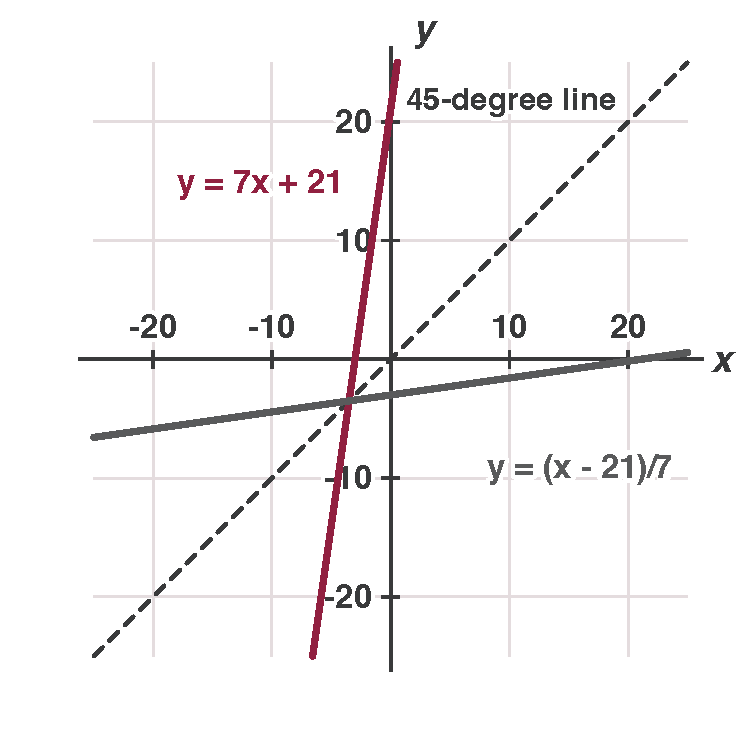
\includegraphics[width=0.45\textwidth,alt={Three lines on the same axes, each running from negative 25 to 25: the steep line y equals 7x plus 21, the flat line y equals x minus 21 over 7, and a dashed 45-degree line y equals x between them; the two solid lines are reflections of each other across the dashed line}]{../../latex/fig/inverse-mirror.pdf}
\end{center}

% Question 6
\item[6.]
\begin{enumerate}
\item[(a)] \[ \frac{d y}{d x}=-6 x^{5}<0 \text{ for } x>0 \]
So the function is strictly decreasing, hence strictly monotonic, and
\[ \frac{d x}{d y}=\frac{1}{d y / d x}=\frac{-1}{6 x^{5}} \]
\item[(b)] \[ \frac{d y}{d x}=20 x^{4}+3 x^{2}+3>0 \text{ for all } x \]
So the function is strictly increasing, hence strictly monotonic, and
\[ \frac{d x}{d y}=\frac{1}{20 x^{4}+3 x^{2}+3} \]
\end{enumerate}
\end{enumerate}
